\section{Prospective test of a spin-adapted frontier configuration extension}
The remaining energy-model error motivated a separate research extension of the
orbital-optimized model. This extension is not substituted for the frozen
production model in the preceding tables. Its native GFN2 ground spatial
orbitals are retained, while the reference one-body levels combine the
projected CAM-B3LYP Fock Rayleigh quotients and qualified full-basis orbital
energies with the unchanged weights $1/2,1/2$. The response exchange scale
remains $\lambda=0.9$; orbital gaps are not multiplied by this scale. The
same prepared reference and native spatial orbitals define the TDA control.
The minimum individually matched native-orbital overlap is greater than
$1-10^{-7}$ in every control calculation. Thus the comparison does not use
full-basis DFT spatial orbitals for TDA.

Optimized, ground-orthogonal ROKS singlets and their paired-double
configurations are supplemented by the spin-adapted configurations of
excitation rank at most two in the highest-two-occupied/lowest-two-virtual
space. An auxiliary CSF with absolute overlap at least 0.7 with a retained
CSF is omitted as redundant. The two four-open-shell singlets are exact
$S=0$ Clebsch--Gordan combinations; they are not broken-symmetry determinants
relabeled as singlets. Their same-occupation block is obtained from the
SU(2)-invariant Heisenberg completion of the quadratic spin functional.
Specifically, with singly occupied site densities $D_i$ and feature moments
$q_i$, $M_{ij}=q_i^{\mathsf T}K_s q_j$, the block is the singlet projection of
\begin{equation}
 E_c+\tfrac12\sum_i M_{ii}+4\sum_{i<j}M_{ij}\mathbf S_i\cdot\mathbf S_j.
\end{equation}
This matches every collinear spin diagonal and the two-spin ROKS limit,
without adding a fitted exchange or excitation-energy parameter. Matrix
elements between different occupations use singular-safe Slater--Condon
algebra and the overlap-weighted mean of the diagonal functional residuals.
This is a distinct approximate state-interaction functional, rather than
an exact multi-determinant form of CAM-B3LYP.

The reported excitation energy is the selected full state-interaction
excited eigenvalue minus the independently stationary ground-functional
energy. This is an explicitly state-specific composite reference: the
auxiliary lowest state-interaction eigenvalue is \emph{not} silently reset
to the ground-functional energy. Its additional lowering is recorded
separately and ranges from 0.050 to 2.428 eV in this pilot. Consequently,
these results cannot be interpreted as gaps between eigenvalues of one
balanced ground-and-excited-state Hamiltonian. No scalar excitation offset
is fitted or applied, but this ground-reference approximation remains a
material modeling limitation.

The excitation-rank hierarchy was examined on nine already exposed states.
Rank two was selected after that development analysis; those nine states
are therefore not blind validation. The candidate was then frozen in commit
\texttt{7666f7a} before its acetone and glyoxal predictions. Both molecules
and their labels had appeared in older campaigns, so this is a prospective
new-model check on historically exposed molecules, not a truly blind test.
Across eleven states the MAE is 0.217 eV and the maximum absolute error is
0.552 eV, compared with 1.163 and 3.660 eV for the identical-kernel native-orbital
TDA control. All eleven states meet the fixed wavefunction-assignment gates.
However, the two prospective states alone give MAE 0.385 eV, compared with
0.420 eV for TDA. Glyoxal is underestimated by 0.552 eV; hence the frozen
0.30-eV-MAE/0.50-eV-maximum accuracy gate is not passed. The much larger
improvement on the exposed development set must not be presented as a
universal correction of lone-pair excitations or as an independently
validated advantage over all calibrated TDA models.

\begin{figure}[htbp]\centering
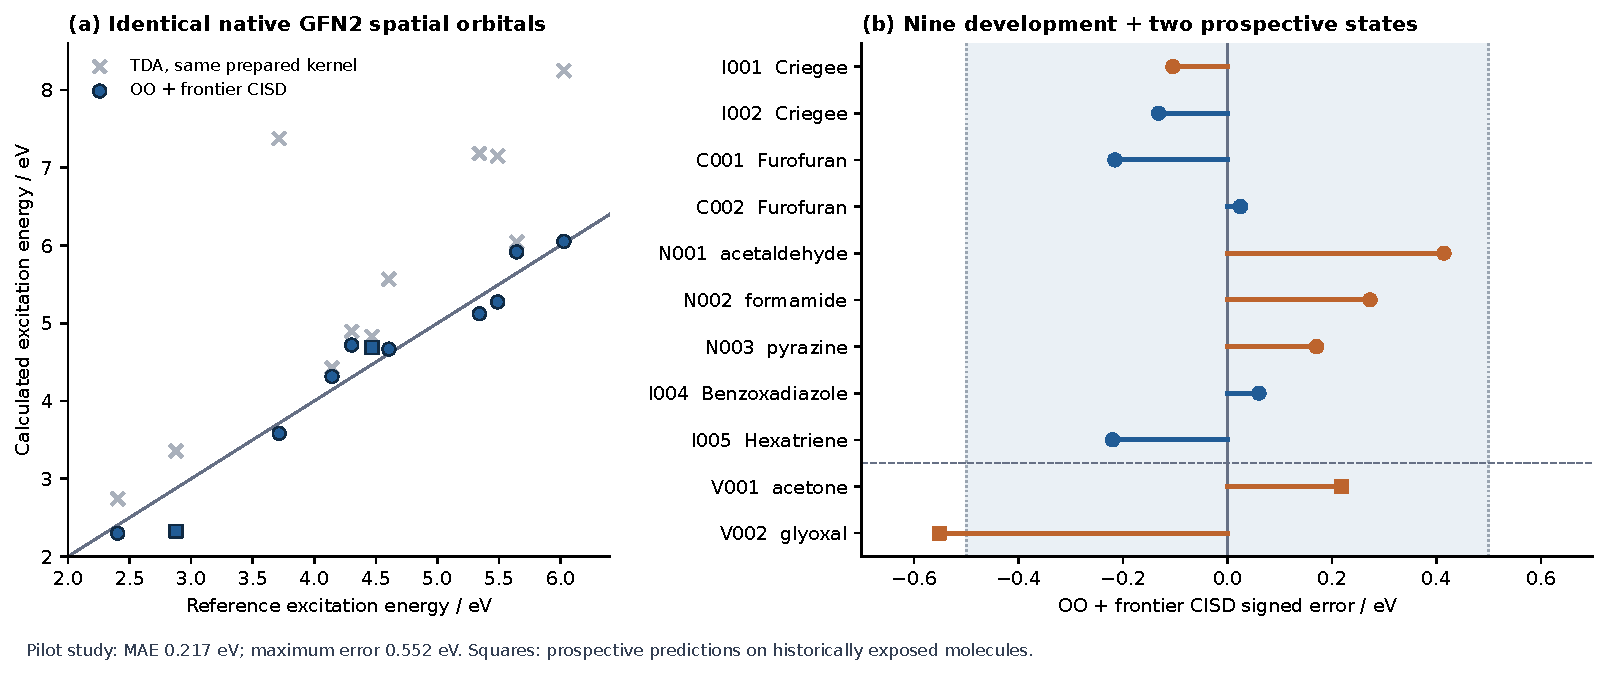
\includegraphics[width=\linewidth]{figures/frontier_cisd_pilot.pdf}
\caption{Exploratory spin-adapted frontier CISD extension. (a) Predictions
and the same-kernel TDA control use the identical native GFN2 ground spatial
orbitals and prepared one-body reference. (b) Signed errors; orange denotes
$n\to\pi^*$ states and blue denotes $\pi\to\pi^*$ states. Squares below the
dashed line identify prospective predictions on historically exposed
molecules. The shaded region is the unchanged $\pm0.5$ eV maximum-error
gate, which glyoxal exceeds.}\label{fig:frontiercisd}
\end{figure}
\begin{table}[htbp]\centering\small
\caption{Pilot vertical excitation energies in eV. The last two rows were
predicted after freezing this candidate.}
\begin{tabular}{llrrr}\hline
ID & Molecule & Reference & OO+CISD & TDA \\ \hline
I001 & Criegee Intermediate & 2.403 & 2.299 & 2.743 \\
I002 & Criegee Intermediate & 3.715 & 3.583 & 7.375 \\
C001 & Furofuran & 5.489 & 5.274 & 7.149 \\
C002 & Furofuran & 6.027 & 6.052 & 8.248 \\
N001 & acetaldehyde & 4.304 & 4.719 & 4.894 \\
N002 & formamide & 5.644 & 5.917 & 6.040 \\
N003 & pyrazine & 4.144 & 4.315 & 4.426 \\
I004 & Benzoxadiazole & 4.606 & 4.666 & 5.565 \\
I005 & Hexatriene & 5.341 & 5.121 & 7.182 \\
V001 & acetone & 4.468 & 4.686 & 4.829 \\
V002 & glyoxal & 2.877 & 2.325 & 3.356 \\
\hline\end{tabular}

\end{table}

The analytic nuclear response is defined for a prepared anchored PES.
Auxiliary canonical orbitals and physical off-diagonal operators are frozen
in the co-rotating orthonormal AO frame; the target ROKS and ground orbitals
retain their complete first and second implicit KKT response. Native diagonal
energies retain explicit geometry and density response. Slater--Condon
matrix elements, overlap metrics, the four-spin block, and the generalized
eigenvalue are differentiated analytically. Auxiliary orbitals are not
re-canonicalized at displaced geometries. This distinction defines the PES
being validated, rather than omitting canonical-orbital response from a
claimed fully re-canonicalized model. Independent displaced, reoptimized
energies are used only to verify the resulting analytic derivatives.

The Criegee target ROKS states can also be recovered from the four canonical
frontier promotions through the ground-program frontend, with no TDA
amplitude reads and no new DFT or SCC call. The exact CSF overlaps with the
retained states differ from unity by less than $10^{-13}$ and the energy
differences are below $4\times10^{-12}$ eV. The corresponding furofuran
recovery has CSF overlaps within $10^{-13}$ of unity and energy differences
below $6\times10^{-12}$ eV. This verifies a TDA-free initialization route
for these four states; it does not establish coverage of CT or Rydberg
states outside the chosen compact orbital space.

Complete analytic Cartesian Hessians of this anchored extension have now
been assembled for both Criegee states (15 coordinates) and both furofuran
states (36 coordinates). Independent reoptimized energies at displacements
of $10^{-3}$ and $5\times10^{-4}$ bohr in two directions verify the
analytic first and second derivatives. Richardson extrapolation of these
validation energies gives maximum gradient errors of $1.12\times10^{-10}$
and $1.31\times10^{-11}$ Hartree/bohr for Criegee and furofuran,
respectively, and directional curvature errors of $1.89\times10^{-7}$ and
$4.03\times10^{-7}$ Hartree/bohr$^2$. The analytic Hessian construction itself
uses no displaced electronic calculation. Raw Hessian asymmetry is at most
$1.16\times10^{-13}$ Hartree/bohr$^2$, and the largest translational sum-rule
residual is $7.20\times10^{-13}$ Hartree/bohr$^2$.

All electronic work for this extension ran on verified Oracle or MAC-STUDIO
hosts. Criegee takes 44.69 s on MAC-STUDIO with two BLAS threads. Furofuran
preserves its already completed sequential columns and completes the remaining
columns with eight independent workers, each using two BLAS threads; that
parallel completion takes 126.83 s. These differently scheduled measurements
are not a common-hardware, common-parallelism scaling benchmark, and the
parallel completion excludes the earlier sequential prefix. They also exclude
one-time DFT-reference preparation. No vertical-energy speed advantage over
TDA is inferred from them.
